\begin{center}
\begin{figure}

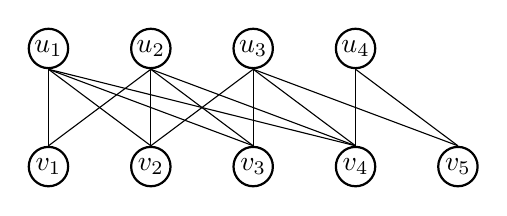
\begin{tikzpicture}[scale=1, 
	every node/.style={circle, draw, minimum size=0.5cm, inner sep=0pt, line width=0.8pt}
]
	
	% Nodes
	\node (u1) at (0,1.5) {$u_1$};
	\node (u2) at (1.3,1.5) {$u_2$};
	\node (u3) at (2.6,1.5) {$u_3$};
	\node (u4) at (3.9,1.5) {$u_4$};

	
	\node (v1) at (0,0) {$v_1$};
	\node (v2) at (1.3,0) {$v_2$};
	\node (v3) at (2.6,0) {$v_3$};
	\node (v4) at (3.9,0) {$v_4$};
	\node (v5) at (5.2,0) {$v_5$};
	
	% Edges
	\draw (u1.south) -- (v1.north);
	\draw (u1.south) -- (v2.north);
	\draw (u1.south) -- (v3.north);
	\draw (u1.south) -- (v4.north);
	\draw (u2.south) -- (v1.north);
	\draw (u2.south) -- (v2.north);
	\draw (u2.south) -- (v3.north);
		\draw (u2.south) -- (v4.north);
	
	\draw (u3.south) -- (v2.north);
	\draw (u3.south) -- (v3.north);
	
	\draw (u3.south) -- (v4.north);
		\draw (u3.south) -- (v5.north);
	

	\draw (u4.south) -- (v4.north);
	\draw (u4.south) -- (v5.north);

\end{tikzpicture}
\caption{An example graph}
\label{fig:ex1} 
\end{figure}
\end{center}